\section{ESN Results}
\label{sec:esn-results}

In this section we show the prediction skill of the more generic ESN
architecture outlined in \cref{subsec:rc}.
Here we use similar metrics as in \cref{sec:nvar-results} to evaluate the ESN
skill, except that we show time averaged quantitative metrics because all of the
ESN predictions are stable for the full 12~hour forecast horizon.
That is, when shown as a single distriubtion rather than a time series, NRMSE is reported as
\begin{linenomath*}\begin{equation}
    \text{NRMSE} = \sqrt{
            \dfrac{1}{\ntime\nstate}\sum_{n=1}^{\ntime}\sum_{i=1}^{\nstate}\left(
        \dfrac{\hat{v}_i(n) - v_i(n)}{SD}
        \right)^2 } \, ,
    \label{eq:total-nrmse} \, ,
\end{equation}\end{linenomath*}
where $\ntime$ consists of the number of timesteps in the trajectory, whether
from the validation or test dataset.
In order to characterize spectral error, we show the KE relative error as in
\cref{sec:nvar-results}.
Additionally, we show the NRMSE in terms of the KE density spectrum as follows
\begin{linenomath*}\begin{equation}
    \text{KE\_NRMSE} = \sqrt{
            \dfrac{1}{\ntime\nk}\sum_{n=1}^{\ntime}\sum_{k=1}^{\nk}\left(
            \dfrac{\hat{E}(n, k) - E(n, k)}{SD(k)}
            \right)^2} \, ,
    \label{eq:ke_nrmse}
\end{equation}\end{linenomath*}
where $\nk$ is the number of spectral coefficients and $SD(k)$ is the temporal
standard deviation of each spectral coefficient throughout the test trajectory.
As in \cref{sec:nvar-results}, all distributions and lineplots indicate
prediction skill from 50 randomly selected initial conditions from an unseen
test dataset.


\subsection{Soft Constraints on Spectral Error}
\label{subsec:esn-ego}

% Here we present ESN results, using mainly the two metrics used to evaluate
% NVAR
It is well known that ESN prediction skill is highly dependent on the global or
``macro-scale'' parameters noted in
\cref{eq:rc-hyperparameters},
\citep<$\esnparams$, e.g.>[]{platt_systematic_2022,lukosevicius_practical_2012}.
Following the success of previous studies in using Bayesian optimization methods
to systematically tune these parameters
\citep{platt_systematic_2022,penny_integrating_2022,griffith_forecasting_2019},
we use the algorithm outlined by \citet{jones_efficient_1998} and implemented by
\citet{bouhlel_python_2019} to find optimal parameter values.

More recently \red{PLATT} showed that constraining these macro-scale
parameters using global invariant properties of the underlying system leads the
optimization algorithm to select parameters that generalize well to unseen test
data.
In their work, the authors were successful in using the largest positive
Lyapunov exponent, and to a lesser extent the fractal dimension of the system.
Because of the focus on resolved scales in this work, we take a similar
approach, but test the effect of constraining the ESN to the KE density
spectral coefficients.
Specifically, we implement the following two stage training process.
At each step, the macro-scale parameters, $\esnparams$, are fixed, and the
``micro-scale'' parameters $\Wout$ are obtained by minimizing \cref{eq:cost}.
This readout matrix is then used to make forecasts from randomly selected
initial conditions from a validation dataset.
The skill of each of these forecasts is captured by the macro-scale cost
function
\begin{linenomath*}\begin{equation}
    \cf_\text{macro}(\esnparams) = \dfrac{1}{\nmacro}
    \sum_{j=1}^{\nmacro}
    \left\{
        \text{NRMSE}(j) + \gamma \text{KE\_NRMSE}(j)
    \right\}
    \label{eq:macro-cost} \, ,
\end{equation}\end{linenomath*}
where NRMSE and KE\_NRMSE are defined in \cref{eq:total-nrmse,eq:ke_nrmse},
$\nmacro$ is the number of forecasts used in the validation set, and $\gamma$ is
a hyperparameter that determintes how much to penalize deviations
from the true KE density spectrum.
The value of $\macrocost$ is then used within the Bayesian optimization
algorithm, which reiterates the whole optimization process with new values for
$\esnparams$ until an optimal value is found or the maximum number of
iterations is reached.
See \red{THE APPENDIX} for more details on our optimization configuration, and
note that we go through this optimization procudure for each unique ESN configuration
throughout \cref{sec:esn-results} (i.e., for each $\nsub$ and each $\gamma$
value).

\cref{fig:rc_qualitative_nsub01} shows a qualitative view of how penalizing the
KE density impacts ESN prediction skill when it operates at the original
timestep of the SQG model (i.e., $\nsub=1$).
At $\gamma=0$, only the ESN parameters are selected based on NRMSE alone, and
the prediction is somewhat blurry.
However, as $\gamma$ increases to $10^{-1}$, the prediction becomes sharper as
the small scale features are seemingly better resolved.

\cref{fig:rc_quantiative_nsub01} gives a quantitative view of how the KE density
penalty changes ESN prediction skill, once again with $\nsub=1$.
The first two panels show that there is a clear tradeoff between NRMSE and KE error:
as $\gamma$ increases the NRMSE decreases but the spectral representation improves.
The final panel in \cref{fig:rc_quantiative_nsub01}
shows that the spatial scales at which the spectral error manifests in these
different solutions.
When $\gamma=0$, the ESN global parameters are chosen to minimize NRMSE, leading
to blurry predictions and a dampened spectrum at the higher wavenumbers,
especially for $|\mathbf{K}| > 2\cdot10^{-3}$~rad~km$^{-1}$.
On the other hand, when $\gamma = 10^{-1}$, the global parameters are chosen to
minimize both NRMSE and KE density error.
In this case, KE relative error is reduced by more than a factor of two and the
spectral bias at higher wavenumbers is much more muted.
However, the tradeoff for this reduced spectral error is larger NRMSE, resulting
from slight mismatches in the position of features in the forecast.
We note that using larger values of $\gamma$ produces similar results to
$\gamma=10^{-1}$.

%However, as time progresses through the 12~hour forecast window,
%the KE relative error increases slightly at the larger spatial scales,
%$|\mathbf{K}| \lessapprox 10^{-3}$~rad~km$^{-1}$ (not shown),
%and this error is what causes NRMSE to be roughly 10\% higher in the case where
%$\gamma=10^{-1}$ than $\gamma=0$.

\begin{figure}
    \centering
    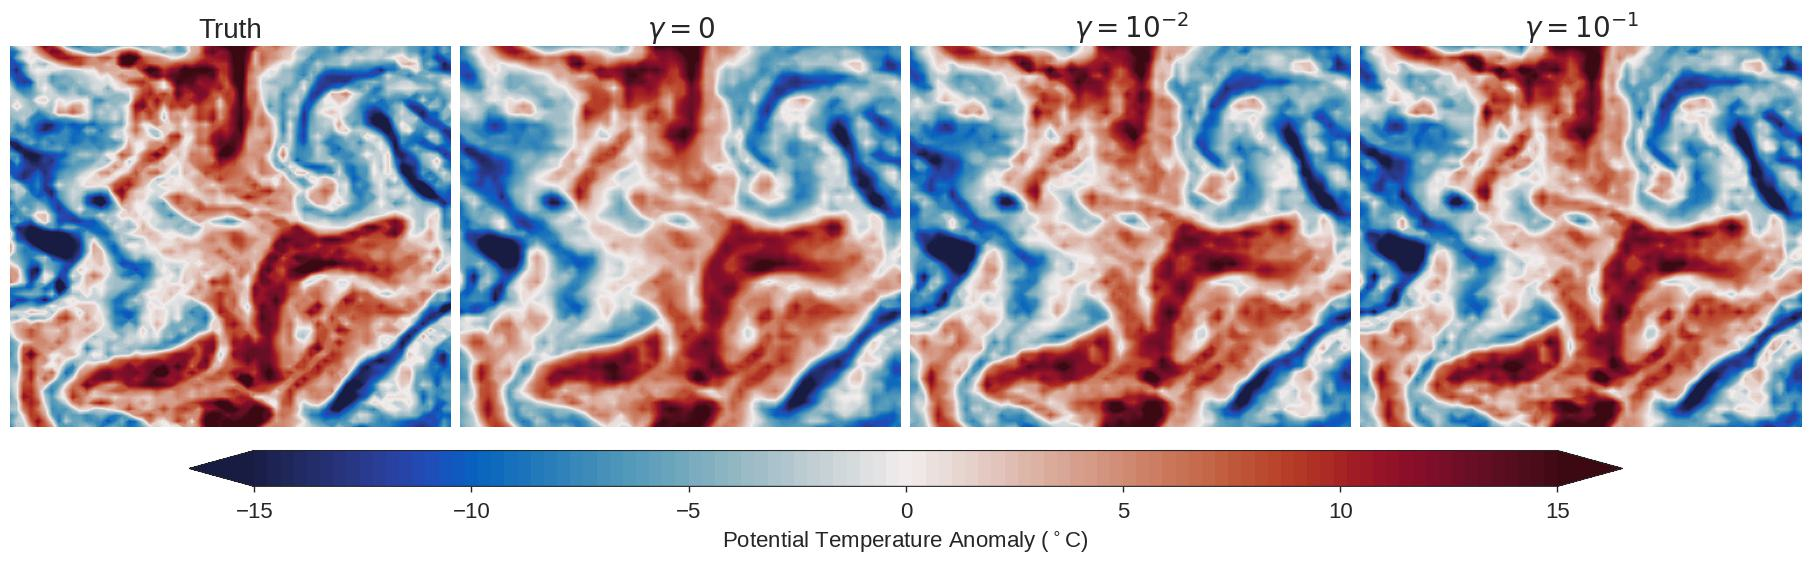
\includegraphics[width=\textwidth]{../figures/rc_qualitative_gamma.jpg}
    \caption{
        One sample prediction from the test dataset, where each panel shows
        potential temperature in the truth (left) and subsequently for
        ESN predictions with parameters optimized using
        $\gamma=\{0, 10^{-2}, 10^{-1}\}$ in \cref{eq:macro-cost}.
        Each panel shows the prediction at a forecast lead time of 4~hours,
        using the same initial conditions as in \cref{fig:nvar_qualitative}.
        Here, the ESN is evaluated at the SQG model timestep, i.e., $\nsub=1$.
    }
    \label{fig:rc_qualitative_nsub01}
\end{figure}

\begin{figure}
    \centering
    \begin{overpic}[width=\textwidth]{../figures/rc_all_nsub01.pdf}
        \put( 6, 27) {(a)}
        \put(40, 27) {(b)}
        \put(72, 27) {(c)}
    \end{overpic}
    \caption{
        Quantitative comparison of ESN predictions at $\nsub=1$ with macro-scale
        parameters
        chosen using different values of $\gamma$ in \cref{eq:macro-cost}.
        NRMSE (\cref{eq:total-nrmse}; a), KE\_NRMSE (\cref{eq:ke_nrmse}; b), and
        KE relative error (\cref{eq:ke_relerr}; c) highlight the tradeoff
        between minimizing NRMSE and spectral bias.
        Note that the KE relative error in (c) is shown at 4~hours to provide
        direct comparison to the snapshots in \cref{fig:rc_qualitative_nsub01}.
    }
    \label{fig:rc_quantiative_nsub01}
\end{figure}



\subsection{The effect of temporal subsampling}
\label{subsec:esn-subsampling}


The NVAR predictions shown in \cref{subsec:nvar-subsampling} indicated that
subsampling the training data increases spectral bias.
However, the architecture was not specifically designed or constrained to
have a good spectral representation of the underlying dynamics.
On the other hand, the previous section (\cref{subsec:esn-ego})
showed that spectral bias can be reduced by optimizing the global ESN parameters
to the true KE density spectrum.
Given these two results, we explore the following question: does temporal subsampling still
increase spectral bias in the more general ESN framework, even when parameters
are chosen to minimize this bias?

\cref{fig:rc_qualitative_gamma0.1} and \cref{fig:rc_quantiative_gamma0.1}
show that even when the macro-scale parameters are chosen to prioritize the KE
density representation (i.e., $\gamma = 0.1$ is fixed),
temporal subsampling does lead to an apparently inescapable spectral bias.
This effect is shown qualitatively in \cref{fig:rc_qualitative_gamma0.1},
where the predictions become
smoother as the temporal subsampling factor, $\nsub$, increases.
The effect is similar to what was seen with NVAR except the blurring effect is
less intense.
Quantitatively, \cref{fig:rc_quantiative_gamma0.1}(b) shows that as $\nsub$
increases, error in KE density spectrum generally increases, while panel (c) shows that this KE
error is concentrated in the small spatial scales,
$|\mathbf{K}| > 2\cdot10^{-3}$~rad~km$^{-1}$.
We note that the degree of spectral bias at $\nsub=16$ is smaller than what was
achieved with NVAR for the same $\nsub$ value, cf. \cref{fig:nvar_ke_vs_lag},
indicating that the optimization was successful in reducing the spectral bias.

\begin{figure}
    \centering
    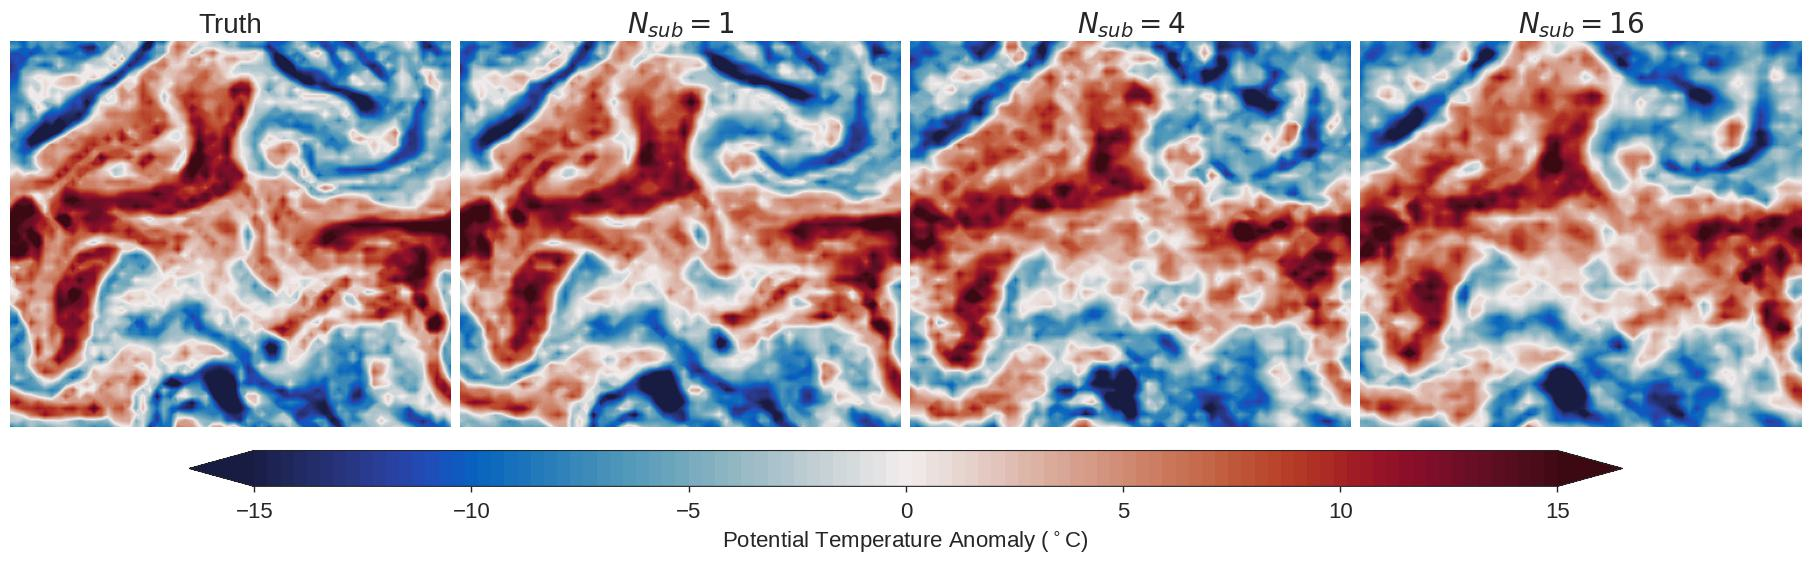
\includegraphics[width=\textwidth]{../figures/rc_qualitative_nsub.jpg}
    \caption{One sample prediction from the test dataset, exactly as in
        \cref{fig:rc_qualitative_nsub01}, except here $\gamma=10^{-1}$ is fixed, and
        the temporal subsampling factor is varied: $\nsub=\{1,4,16\}$.
    }
    \label{fig:rc_qualitative_gamma0.1}
\end{figure}

\begin{figure}
    \centering
    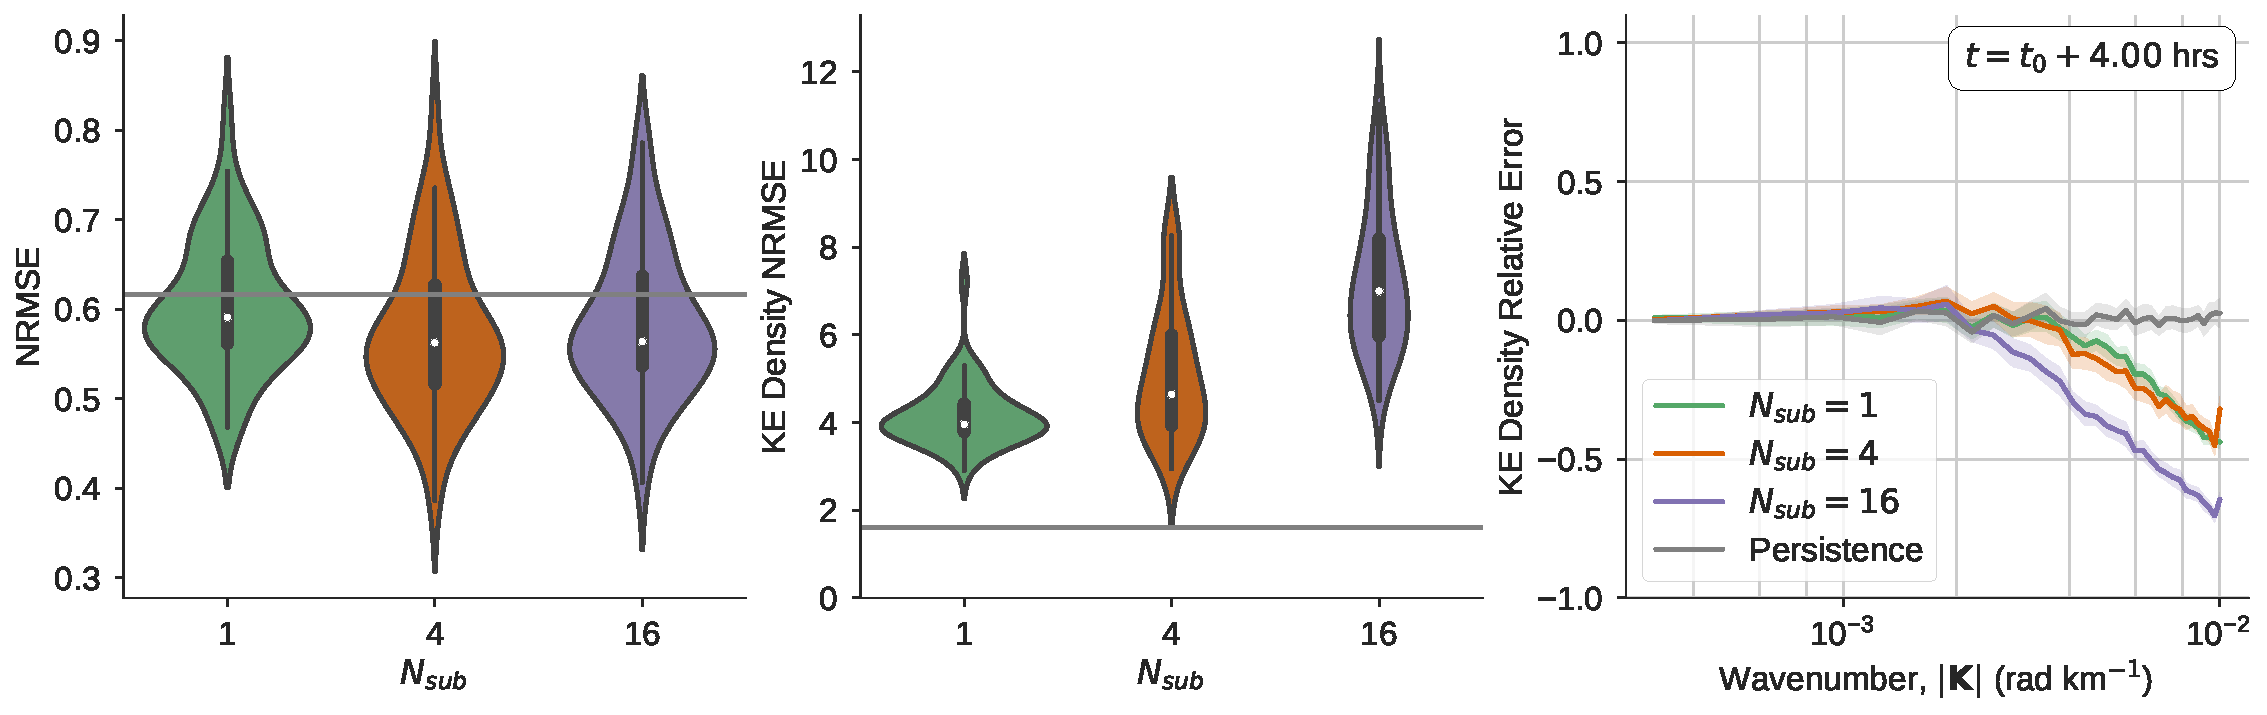
\includegraphics[width=\textwidth]{../figures/rc_all_gamma0.1.pdf}
    \caption{Quantitative comparison of ESN predictions, showing
        NRMSE (a), KE\_NRMSE (b), and KE relative error (c), exactly as in
        \cref{fig:rc_quantiative_nsub01}, except here $\gamma=10^{-1}$ is fixed,
        and the temporal subsampling factor is varied: $\nsub=\{1,4,16\}$.
    }
    \label{fig:rc_quantiative_gamma0.1}
\end{figure}

Interestingly, there is little difference between NRMSE obtained by the ESNs at
different $\nsub$ values.
Additionally, \cref{fig:rc_quantiative_gamma0.0} shows that there is little
difference in NRMSE even when $\gamma=0$, i.e., when NRMSE is the only criterion
for parameter selection.
Therefore, if the goal is to simply produce a prediction with minimal RMSE over a
12~hour window, then it is beneficial to subsample the data in time because of
the improvements in computational efficiency.
However, if the goal is to represent all spatial scales in the data as well as
possible, then NRMSE alone is not a good criterion for model selection.
This assertion is corroborated by the discussion in \cref{subsec:esn-ego}, and
with the fact that when $\gamma=0$ there is little difference in KE error
no matter how the data are subset, even though this difference is stark when
KE density is more appropriately prioritized.

\begin{figure}
    \centering
    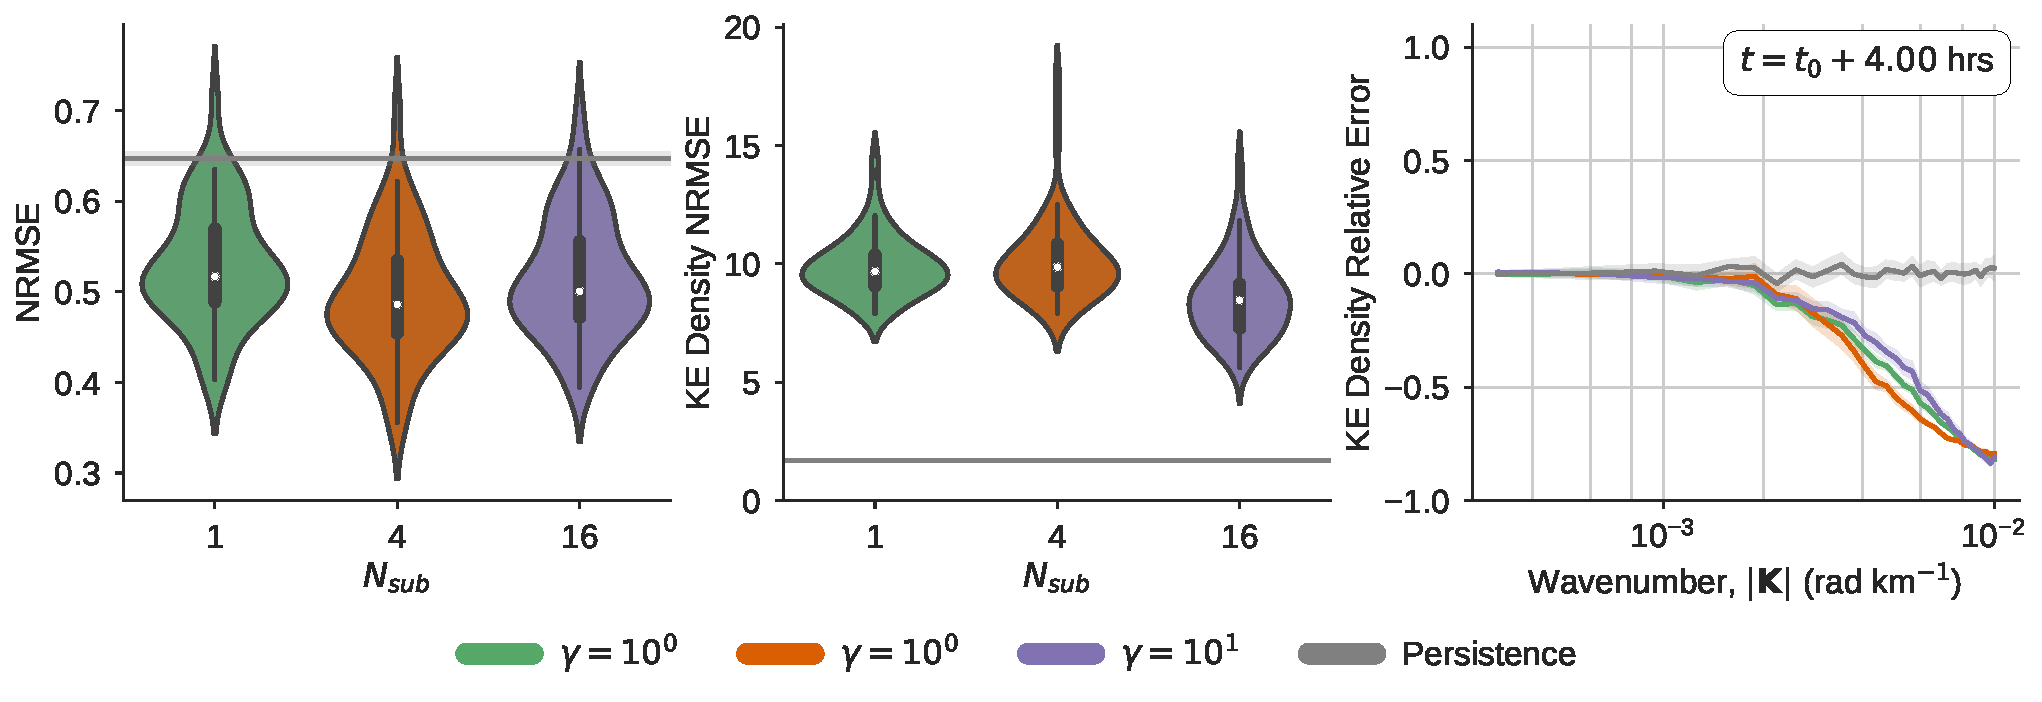
\includegraphics[width=\textwidth]{../figures/rc_all_gamma0.0.pdf}
    \caption{Same as \cref{fig:rc_quantiative_gamma0.1}, except here $\gamma=0$.}
    \label{fig:rc_quantiative_gamma0.0}
\end{figure}

\subsection{Impact of reservoir size}
\label{subsec:esn-size}

The size of the reservoir, $\nhidden$, determines the
memory capacity available to the ESN
\citep{jaeger_echo_2001,lukosevicius_practical_2012}.
For systems with high dimensional input signals, it is crucial to use a ``large
enough'' reservoir to afford the memory capacity necessary for accurate
predictions \citep{hermans_memory_2010}.
In all the preceding sections we fixed $\nhidden=6,000$ at each local group,
where for reference each local group has an input dimension of
$\ninputstate=200$ and an output dimension of $\nstate=128$.
Here, we briefly address the effect of doubling the reservoir size,
while keeping the input and output dimensions constant, in order to test how
sensitive our conclusions are on this crucial hyperparameter.
Due to the computational expense of the parameter optimization discussed in
\cref{subsec:esn-ego}, we only perform this experiment for $\nsub=16$.

The impact of doubling $\nhidden$ on prediction skill is shown in
\cref{fig:esn-size}, where for the sake of brevity we only show results for the
case when $\gamma=0.1$ in \cref{eq:macro-cost}.
Panel (a) shows that the larger reservoir actually increases the NRMSE slightly.
However, panels (b) and (c) show that this increase is due to the improved
representation of KE density.
The improvement in KE\_NRMSE is nearly proportional to the improvement achieved by increasing
the temporal resolution of the data.
That is, doubling the reservoir size reduces the average KE\_NRMSE by 14\%,
while increasing the temporal resolution of the data by a factor of 4 reduces
the KE\_NRMSE by 30\%.

\begin{figure}
    \centering
    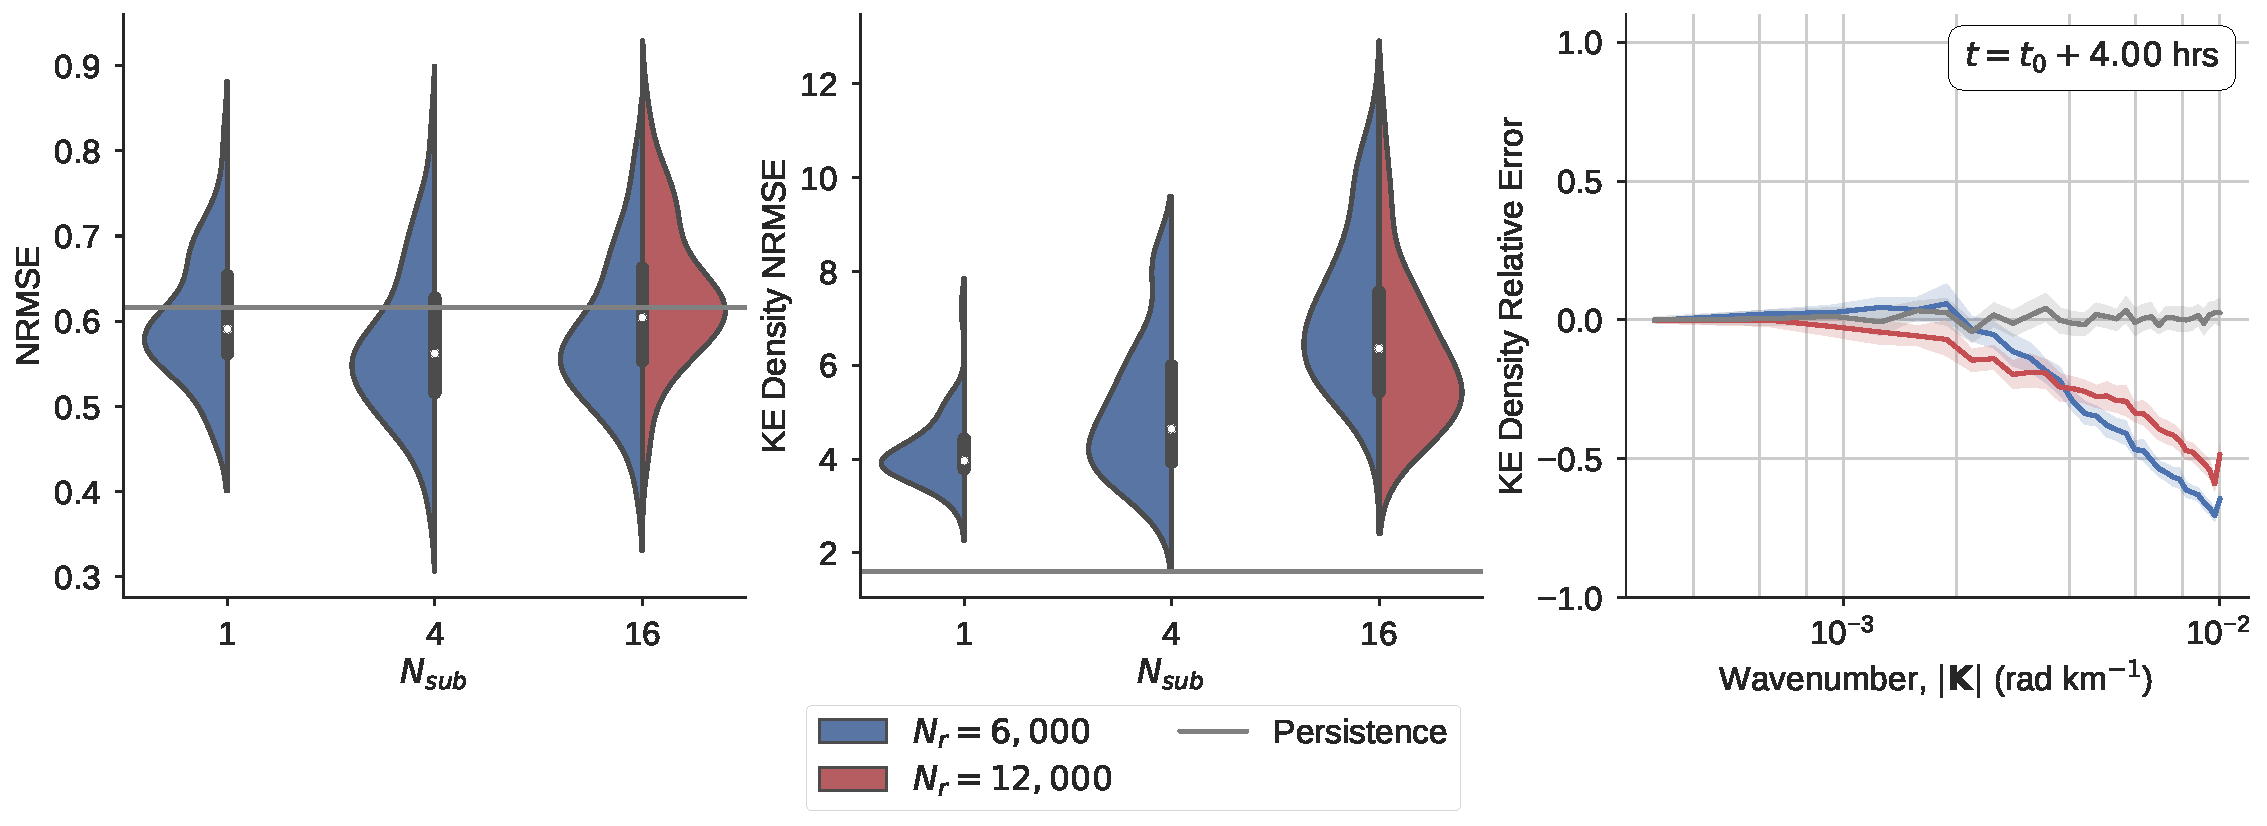
\includegraphics[width=\textwidth]{../figures/rc_reservoir_size.pdf}
    \caption{The impact of doubling the reservoir size from $\nhidden=6,000$ to
        $\nhidden=12,000$ on NRMSE (a), KE\_NRMSE (b), and KE relative error (c).
        Here $\gamma=0.1$.
    }
    \label{fig:esn-size}
\end{figure}
